\documentclass{article}
\usepackage{fullpage,graphicx}
\usepackage{amsmath,amsfonts,amsthm,amssymb,multirow,xcolor}
\usepackage{algorithmic}
\usepackage[ruled,vlined,commentsnumbered,titlenotnumbered]{algorithm2e}
\usepackage{minted}
\usepackage{multicol}
\usepackage{tikz}
\usetikzlibrary{positioning}


\usepackage{pgfplots}
\pgfplotsset{compat=1.10}
\usetikzlibrary{shapes.geometric,arrows,fit,matrix,positioning}
\tikzset
{
  treenode/.style = {circle, draw=black, align=center, minimum size=1cm},
  subtree/.style  = {isosceles triangle, draw=black, align=center, minimum height=0.5cm, minimum width=1cm, shape border rotate=90, anchor=north}
}

\begin{document}
\noindent
CS 161 \hfill \textbf{Homework 4} \newline 
Summer 2018 \hfill \textbf{Due:} Thursday 8/2 at 5 p.m. on Gradescope

\noindent\rule{\linewidth}{0.4pt}

\section*{Exercises}

Exercises should be completed \textbf{on your own}.

\noindent\rule{\linewidth}{1.0pt}

\noindent
\textbf{Drawing graphs:} You might try \texttt{http://madebyevan.com/fsm/}
which allows you to draw graphs with your mouse and convert it into \LaTeX\, code:

\begin{center}
  %%%%%%% GENERATED AUTOMATICALLY BY madebyevan.com/fsm/
  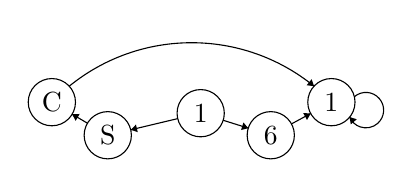
\begin{tikzpicture}[scale=0.1]
    \tikzstyle{every node}+=[inner sep=0pt]
    \draw [black] (26.7,-13.3) circle (3);
    \draw (26.7,-13.3) node {C};
    \draw [black] (45.6,-14.7) circle (3);
    \draw (45.6,-14.7) node {$1$};
    \draw [black] (33.8,-17.5) circle (3);
    \draw (33.8,-17.5) node {S};
    \draw [black] (54.5,-17.5) circle (3);
    \draw (54.5,-17.5) node {$6$};
    \draw [black] (62.2,-13.3) circle (3);
    \draw (62.2,-13.3) node {$1$};
    \draw [black] (42.68,-15.39) -- (36.72,-16.81);
    \fill [black] (36.72,-16.81) -- (37.61,-17.11) -- (37.38,-16.14);
    \draw [black] (31.22,-15.97) -- (29.28,-14.83);
    \fill [black] (29.28,-14.83) -- (29.72,-15.67) -- (30.23,-14.8);
    \draw [black] (48.46,-15.6) -- (51.64,-16.6);
    \fill [black] (51.64,-16.6) -- (51.03,-15.88) -- (50.73,-16.84);
    \draw [black] (57.13,-16.06) -- (59.57,-14.74);
    \fill [black] (59.57,-14.74) -- (58.62,-14.68) -- (59.1,-15.56);
    \draw [black] (28.907,-11.271) arc (129.11449:50.88551:24.638);
    \fill [black] (59.99,-11.27) -- (59.69,-10.38) -- (59.06,-11.15);
    \draw [black] (65.108,-12.614) arc (131.00538:-156.99462:2.25);
    \fill [black] (64.51,-15.19) -- (64.66,-16.12) -- (65.42,-15.47);
  \end{tikzpicture}
\end{center}
\rule{\linewidth}{0.4pt}

\begin{enumerate}
  \item \textbf{(Fun with Dijkstra)} \textbf{(8 pt.)}

    Let $G = (V,E)$ be a weighted directed graph. For the rest of this problem,
    assume that $s, t \in V$ and that \textbf{there exists a directed path from
    $s$ to $t$}. The weights on $G$ could be anything: \textbf{negative, zero, or
    positive.}

    For the rest of this problem, refer to the implementation of Dijkstra's 
    algorithm given by the pseudocode below.

\begin{minted}[mathescape,
               linenos]{python}
def dijkstra_st_path(G, s, t):
  for all v in V: set d[v] = Infinity
  for all v in V: set p[v] = None 
  
  # we will use p to reconstruct the shortest s-t path at the end
  d[s] = 0
  F = V
  D = []
  while F is not empty:
    x = vertex v in F such that d[v] is minimized
    for y in x.outgoing_neighbors:
      d[y] = min(d[y], d[x] + weight(x,y))
      if d[y] was changed in the previous line: set p[y] = x
    F.remove(x)
    D.add(x)
        
  // use p to reconstruct the shortest s-t path
  path = [t]
  current = t
  while current != s:
    current = p[current]
    add current to the front of the path
  return path, d[t]
\end{minted}

    Notice that the pseudocode above differs from the pseudocode in the notes. The
    variable \verb|p| maintains the ``\textbf{p}arents'' of the vertices in the
    shortest s-t path, so it can be reconstructed at the end.

    \begin{enumerate}
      \item \textbf{(1 pt.)} Step through \texttt{dijkstra\_st\_path}$(G,s,t)$ on
        the graph $G$ shown below. Complete the table below to show what the arrays
        \texttt{d} and \texttt{p} are at each step of the algorithm, and indicate
        what path is returned and what its cost is.

\begin{center}
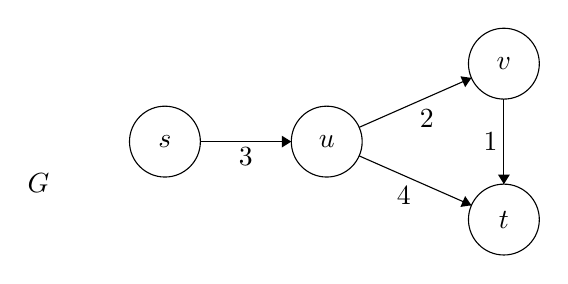
\begin{tikzpicture}[scale=0.15]
\tikzstyle{every node}+=[inner sep=0pt]
\draw [black] (20.7,-26.5) circle (3);
\draw (20.7,-26.5) node {$s$};
\draw [black] (34.4,-26.5) circle (3);
\draw (34.4,-26.5) node {$u$};
\draw [black] (49.4,-19.9) circle (3);
\draw (49.4,-19.9) node {$v$};
\draw [black] (49.4,-33.1) circle (3);
\draw (49.4,-33.1) node {$t$};
\draw [black] (23.7,-26.5) -- (31.4,-26.5);
\fill [black] (31.4,-26.5) -- (30.6,-26) -- (30.6,-27);
\draw (27.55,-27) node [below] {$3$};
\draw [black] (37.15,-25.29) -- (46.65,-21.11);
\fill [black] (46.65,-21.11) -- (45.72,-20.97) -- (46.12,-21.89);
\draw (42.88,-23.71) node [below] {$2$};
\draw [black] (49.4,-22.9) -- (49.4,-30.1);
\fill [black] (49.4,-30.1) -- (49.9,-29.3) -- (48.9,-29.3);
\draw (48.9,-26.5) node [left] {$1$};
\draw [black] (37.15,-27.71) -- (46.65,-31.89);
\fill [black] (46.65,-31.89) -- (46.12,-31.11) -- (45.72,-32.03);
\draw (40.92,-30.31) node [below] {$4$};
\node at (10,-30) {$G$};
\end{tikzpicture}
\end{center}

        \textbf{[We are expecting the table below filled out, as well as the final
        shortest path and its cost. No further justification is required.]}

%%%%%%%%%%%%%%%%%%%%%%%%%%%%%%%%%%%%%%%%%%%%%%%%%%%%%%%%%%%%%%%%%%%%%%%%%%%%%%%%
%%%%%%%% TABLE: Fill in your answers between the & symbols below  if    %%%%%%%%
%%%%%%%% you wish to take this LaTeX code for your solution.            %%%%%%%%
%%%%%%%%%%%%%%%%%%%%%%%%%%%%%%%%%%%%%%%%%%%%%%%%%%%%%%%%%%%%%%%%%%%%%%%%%%%%%%%%

        \begin{center}
          \def\arraystretch{1.5}
          \newcommand{\td}{\texttt{d}}
          \newcommand{\tp}{\texttt{p}}
          \begin{tabular}{|p{6cm}||c|c|c|c||c|c|c|c|}
          \hline
          & \td[$s$] & \td[$u$] & \td[$v$] & \td[$t$] & \tp[$s$] & \tp[$u$] & \tp[$v$] & \tp[$t$] \\
          \hline
          When entering the first while loop for the first time, the state is:&
          0 & $\infty$ & $\infty$ & $\infty$ & None & None & None & None \\
          \hline
          Immediately after the first element of $D$ is added, the state is: &
          0 & $3$ & $\infty$ & $\infty$ & None & s & None & None \\
           \hline
          Immediately after the second element of $D$ is added, the state is: &
           & & & & & & & \\
           \hline
          Immediately after the third element of $D$ is added, the state is: &
           & & & & & & & \\
           \hline
          Immediately after the fourth element of $D$ is added, the state is: &
           & & & & & & & \\
           \hline
          \end{tabular}
        \end{center}

%%%%%%%% END TABLE %%%%%%%%

      \item \textbf{(1 pt.)} \textbf{Prove or disprove}: In every such graph $G$,
        the shortest path from $s$ to $t$ exists.  Here, a \em path \em from $s$
        to $t$ is formally defined as a sequence of edges
        \[ (u_0,u_1), (u_1, u_2), (u_2,u_3), \ldots, (u_{M-1}, u_M)\]
        such that $u_0 = s$, $u_M = t$, and $(u_i, u_{i+1}) \in E$ for all
        $i=0,\ldots,M-1$.  A \em shortest path \em is a path
        $((u_0,u_1),\ldots,(u_{M-1},u_M))$ such that
        \[ \sum_{i=0}^{M-1} \mathrm{weight}(u_i,u_{i+1}) \leq  \sum_{i=0}^{M'-1} \mathrm{weight}(u'_i, u_{i+1}')\]
        for all paths $((u'_0, u'_1),\ldots, (u'_{M'-1}, u'_{M'}))$.

      \item \textbf{(2 pt.)} \textbf{Prove or disprove}: In every such graph $G$
        in which the shortest path from $s$ to $t$ exists,
        \texttt{dijkstra\_st\_path}$(G, s,t)$ returns a shortest path between $s$
        and $t$ in $G$.

      \item \textbf{(2 pt.)} \textbf{Prove or disprove}: In every such graph $G$
        in which there is a negative-weight edge, and for all $s$ and $t$,
        \texttt{dijkstra\_st\_path}$(G, s,t)$ does not return a shortest path
        between $s$ and $t$ in $G$.
  
      \newpage

      \item \textbf{(2 pt.)} Your friend offers the following way to patch up
        Dijkstra's algorithm to deal with negative edge weights. Let $G$ be a
        weighted graph, and let $w^*$ be the smallest weight that appears in $G$.
        (Notice that $w^*$ may be negative). Consider a graph $G' = (V,E')$ with
        the same vertices, and such that $E'$ is as follows: for every edge
        $e \in E$ with weight $w$, there is an edge $e' \in E'$ with weight
        $w - w^*$. Now all of the weights in $G'$ are non-negative, so we can
        apply Dijkstra's algorithm to that:

        \begin{verbatim}
modified_dijkstra(G,s,t):
  Construct G' from G as above.
  return dijkstra_st_path(G',s,t)
        \end{verbatim}
       
        \textbf{Prove or disprove}: Your friend's approach will always correctly
        return a shortest path between $s$ and $t$ if it exists.
    \end{enumerate}
  \newpage
\end{enumerate}

\section*{Problems}

You can collaborate with your classmates about the problems. However:

\begin{itemize}
  \item Try the problems on your own \textit{before} collaborating.
  \item Write up your solutions yourself, in your own words.  You should never
    share your typed-up solutions with your collaborators.
  \item If you collaborated, list the names of the students you collaborated
    with at the beginning of each problem.
\end{itemize}

\noindent\rule{\linewidth}{1.0pt}

\begin{enumerate}
    \item \textbf{(Currency Exchange)} \textbf{(9 pt.)}
    \begin{enumerate}
      \item \textbf{(3 pt.)} Suppose the economies of the world use a set of
        currencies $C_1,\ldots,C_n$; think of these as dollars, pounds, Bitcoin,
        etc. Your bank allows you to trade each currency $C_i$ for any other
        currency $C_j$, and finds some way to charge you for this service.
        Suppose that for each ordered pair of currencies $(C_i,C_j)$, the bank
        charges a flat fee of $f_{ij} > 0$ dollars to exchange $C_i$ for $C_j$
        (regardless of the quantity of currency being exchanged).

        Devise an efficient algorithm which, given a starting currency $C_s$, a
        target currency $C_t$, and a list of fees $f_{ij}$ for all
        $i,j \in \{1,\ldots,n\}$, computes the cheapest way (that is, incurring
        the least in fees) to exchange all of our currency in $C_s$ into
        currency $C_t$. Also, justify the correctness of your algorithm and its
        runtime.

        \textbf{[We are expecting a description or pseudocode of your algorithm
        as well as a brief justification of its correctness and runtime.]}

      \item \textbf{(3 pt.)} Consider the more realistic setting where the bank
        does not charge flat fees, but instead uses exchange \emph{rates}. In
        particular, for each ordered pair $(C_i,C_j)$, the bank lets you trade
        one unit of $C_i$ for $r_{ij} > 0$ units of $C_j$. Devise an efficient
        algorithm which, given starting currency $C_s$, target currency $C_t$,
        and a list of rates $r_{ij}$, computes a sequence of exchanges that
        results in the greatest amount of $C_t$.  Justify the correctness of
        your algorithm and its runtime. [Hint: How can you turn a product of
        terms into a sum?  Take logarithms.]

      \item \textbf{(3 pt.)} Due to fluctuations in the markets, it is
        occasionally possible to find a sequence of exchanges that lets you
        start with currency A, change into currencies, B, C, D, etc., and then
        end up changing back to currency A in such a way that you end up with
        more money than you started with---that is, there are currencies
        $C_{i_1},\ldots,C_{i_k}$ such that
        \[ r_{i_1 i_2} \times r_{i_2 i_3} \times \cdots \times r_{i_{k-1} i_k} \times r_{i_k i_1} > 1 . \]
        Devise an efficient algorithm that finds such an anomaly if one exists.
        Justify the correctness of your algorithm and its runtime.
    \end{enumerate}

  \newpage

  \item \textbf{(Allocating Surfboards)} \textbf{(8 pt.)}
  
    A group of $n$ friends have respective heights $h_1 < h_2 < ... < h_n$ (where
    $h_i$ is the height of friend i). They decide to go surfing and need to rent
    surfboards. The surf shop has a rack with $m > n$ surfboards ordered by
    lengths $s_1 < s_2 < ... < s_m$. In small/clean waves, the ideal surfboard has
    the same length as your height. Help us figure out a good allocation of the
    boards.

    Formally, an allocation of surfboards is a function
    $f : \{1, ..., n\} \rightarrow \{1, ..., m\}$ that maps each surfer to a
    surfboard. More precisely, $f(2) = 3$ means that surfer 2 (with height $h_2$)
    receives surfboard 3 (with length $s_3$). An allocation $f$ is optimal if it
    minimizes the quantity $\sum_{k=1}^n | h_k - s_{f(k)} |$. That is, an
    allocation is optimal if it minimizes the sum of the discrepancies of height
    between the surfers and their surfboards.

    Let $A[n, m]$ denote this minimal difference.

    \begin{enumerate}
      \item \textbf{(2 pt.)} Let $A[i, j]$ denote the sum of discrepancies of an
        optimal allocation of the first $j$ surfboards to the first $i$ surfers
        $(j \geq i)$. Prove that, if surfboard $j$ is used in an optimal
        allocation, then there is an optimal allocation in which it is allocated
        to surfer $i$.

        Note: There might be multiple optimal allocations. This part asks you to
        show that if the longest board is used, then it might as well go to the
        tallest surfer.

        [\textbf{We are expecting: A formal proof of your answer}]

      \item \textbf{(2 pt.)} Deduce a recurrence relation between
        $A[i, j], A[i, j - 1]$ and $A[i - 1, j - 1]$. 

        Hint: Consider two cases, according to whether surfboard $j$ is used or
        not.

        \textbf{[We are expecting: A statement of the recurrence as well as a
        short explanation of it.]}

      \item \textbf{(3 pt.)} Design a dynamic programming algorithm that computes
        $A[n, m]$ and also outputs the optimal allocation.

        \textbf{[We are expecting: A description of a procedure or pseudocode of
        an algorithm.]}
	
      \item \textbf{(1 pt.)} What is the runtime of your algorithm? Prove your
        answer.

        \textbf{[We are expecting: An informal analysis of the runtime.]}

    \end{enumerate}
\end{enumerate}

\end{document}